\documentclass[10pt]{beamer}
\usetheme{metropolis}
\metroset{block=fill}

\newcommand{\relu}[0]{\mathsf{ReLU}}

\usepackage[sfdefault]{FiraSans}
\renewcommand*\oldstylenums[1]{{\firaoldstyle #1}}

\usepackage[T1]{fontenc}
\usepackage{amsmath,amssymb,mathtools}
\newcommand{\set}[1]{\left\{ #1 \right \}}

\usepackage{multimedia}
\usepackage{graphicx}
\definecolor{navyblue}{RGB}{0,0,128}
\tikzset{
    descr/.style={
        fill=white,
        inner sep=2.5pt
    },
    connector/.style={
     -latex,
     font=\normalsize
    },
    rectangle connector/.style={
        connector,
        to path={(\tikztostart) -- ++(#1,0pt) \tikztonodes |- (\tikztotarget) },
        pos=0.5
    },
    rectangle connectorh/.style={
        connector,
        to path={(\tikztostart) -- ++(0pt,#1)  -| (\tikztotarget) \tikztonodes },
        pos=0.5
    },
    rectangle connector/.default=-2cm,
    straight connector/.style={
        connector,
        to path=--(\tikztotarget) \tikztonodes
    }
}

%\usetikzlibrary{shapes,arrows,positioning,fit,chains,shapes.multipart,calc}
\tikzstyle{line}=[draw,-latex']

\newlength{\mfw}
\setlength{\mfw}{0.4\linewidth}


\newcommand\blfootnote[1]{%
  \begingroup
  \renewcommand\thefootnote{}\footnote{#1}%
  \addtocounter{footnote}{-1}%
  \endgroup
}


\begin{document}

\title{Formal Verification of Neuro-symbolic Multi-agent Systems}
\author{ Panagiotis Kouvaros} 
\institute[U of X]
{
Department of Computing, Imperial College London, UK \\ \\

Joint work with Michael Akintunde, Francesco Belardinelli, Ioana
Boureanu,  Elena Botoeva, Jan Kronqvist,
Alessio Lomuscio, Ruth Misener
}
\date{}

%%%%%%%%%%%%%%%%%%%%%%%%%%%%%%%%%%%%%%%%%%%%%%%%%%%%%%%%%%%%%%%%%%%%%%%%%%%%%%

\begin{frame}
  	\maketitle
\end{frame}

%%%%%%%%%%%%%%%%%%%%%%%%%%%%%%%%%%%%%%%%%%%%%%%%%%%%%%%%%%%%%%%%%%%%%%%%%%%%%%

\begin{frame}{AI safety}

	Rapid progress in AI in diverse domains, including natural
	language processing, computer vision, autonomous vehicles.

	\vspace{2em}

	Increasing prevalence of AI to society (healthcare,
	transportation, finance, e-commerce).


	\vspace{2em}

	Potentially AI will be \alert{highly beneficial} to society.


	\vspace{2em}

	Yet, its inherent \alert{lack of explainability} and
	\alert{fragility} hinders the its adoption by society.
\end{frame}	
	
%%%%%%%%%%%%%%%%%%%%%%%%%%%%%%%%%%%%%%%%%%%%%%%%%%%%%%%%%%%%%%%%%%%%%%%%%%%%%%

\begin{frame}{AI perils}

\begin{center}
	\includegraphics[width=\textwidth]{tesla.png}
\end{center}

\end{frame}

%%%%%%%%%%%%%%%%%%%%%%%%%%%%%%%%%%%%%%%%%%%%%%%%%%%%%%%%%%%%%%%%%%%%%%%%%%%%%%

\begin{frame}{Research aim}
		
	The development of methods to show that AI \alert{robustly behaves as
	intended}.

\end{frame}

%%%%%%%%%%%%%%%%%%%%%%%%%%%%%%%%%%%%%%%%%%%%%%%%%%%%%%%%%%%%%%%%%%%%%%%%%%%%%%

\begin{frame}{Formal verification of AI}
	
	Formal verification has long been used for the certification of
	safety-critical systems.

	\begin{block}{Formal verification problem}
			\begin{large}
		
		\[
			\mathcal M_S \models \varphi_P ?
		\]

			\end{large}

	\end{block}

	\alert{$\mathcal{M}_S$} is a semantic model of a MAS $S$
	\begin{center}
	\documentclass{standalone}

\usepackage[T1]{fontenc}
\usepackage{amsmath,amssymb,mathtools}
\newcommand{\set}[1]{\left\{ #1 \right \}}

\usepackage{graphicx}
\definecolor{navyblue}{RGB}{0,0,128}
\begin{document}

	\begin{tikzpicture}[node distance=2.3cm,  minimum
	  height=0.7cm,font=\scriptsize]

	  \path[fill=white]  (7,-1.7) -- (5.7,1.4) -- (-1.8,1.4)
	  -- (-1.8,-1.2) -- (5.7,-1.2) -- (7,-1.7);


	 \node[draw=navyblue,fill=navyblue!5!white,rectangle,xshift=0cm]
	 (1) {Perception};

	\node[draw=navyblue, fill=navyblue!5!white,rectangle, right of=1,
	xshift=0em, yshift=0cm, inner ysep=0.15cm] (2)
	{Reasoning};

	\node[above of=2, xshift=-1em, yshift=-1.6cm] (l)
	{\includegraphics[width=0.5cm]{agent.png}};

	\node[right of=l, xshift=-4.5em] (l2) {Agent};

	\node[draw=navyblue, fill=navyblue!5!white,rectangle, right
	of=2,xshift=0em, yshift=0cm]  (3) {Action};

	\node[draw=navyblue, fill=navyblue!5!white,rectangle, above of=1,
	xshift=6.7em,yshift=0.3cm,align=left] (5) {Environment};

	%\node[draw=navyblue, fill=navyblue!5!white,rectangle, right
	%of=5] (4) {Plant};
		
	%\node[fit=(1)(2)(3)(l)(l2), line width=0.01em, dashed, rounded corners,
	%inner sep=0.2cm] (s) {};


	  %\node[draw=navyblue,fill=navyblue!5!white,rectangle, 
	  %inner ysep=0.15cm, right of=s, xshift=5cm] (0) {\includegraphics[width=5.5cm]{mas.png}};


	\draw[->,thick] (1) -- (2);	
	\draw[->,thick] (2) -- (3);	
	%\draw[->,thick] (3.north) |- (4.east);	
	\draw[<-,thick] (5) -| (3);
	%\draw[-latex,thick] (4.west) to (5);
	\draw[->,thick] (5.west) -| (1.north);
	
	%\draw[-,line width=0.03cm,green,dotted] (5.7,1.4) -- (7,-1.7);
	%\draw[-,line width=0.03cm,green,dotted] (5.7,1.4) -- (-1.8,1.4);
	%\draw[-,line width=0.03cm,green,dotted] (-1.8,1.3) -- (-1.8,-1.2);
	%\draw[-,line width=0.03cm,green,dotted] (-1.8,-1.2) -- (5.7,-1.2);
	%\draw[-,line width=0.03cm,green,dotted] (5.7,-1.2) -- (7,-1.7);

	\draw[draw=black,rounded corners] (-1.3,-1) rectangle ++(6.9,2.2);	
	\draw[draw=black,rounded corners] (-1.2,-0.9) rectangle ++(6.7,2);	
	%\draw[draw=black,rounded corners] (-1.6,-0.5) rectangle ++(0.3,1);	
	%\draw[draw=black,rounded corners] (5.6,-0.5) rectangle ++(0.3,1);	


	%\node[fit=(0)(1)(4), draw, navyblue, line width=0.1cm, dashed, rounded corners,
	%inner sep=0.2cm] (s) {};


  \end{tikzpicture}
\end{document}
%%% Local Variables:
%%% mode: latex
%%% TeX-master: "deliverable-wp1.1-m18"
%%% fill-column: 79
%%% End:
	
	\end{center}
	\alert{$\phi_P$} is a logical formula (temporal, epistemic,
	ATL, \ldots) encoding a specification~$P$ for the MAS $S$ under
	analysis

	% Problem has many instantiation woth of consideration.

\end{frame}

%%%%%%%%%%%%%%%%%%%%%%%%%%%%%%%%%%%%%%%%%%%%%%%%%%%%%%%%%%%%%%%%%%%%%%%%%%%%%%

\begin{frame}{Noteworthy instantiations}
%\begin{columns}
%\begin{column}{0.3\textwidth}
	%\begin{block}{Symbolic agents}
		%\documentclass{standalone}

\usepackage[T1]{fontenc}
\usepackage{amsmath,amssymb,mathtools}
\newcommand{\set}[1]{\left\{ #1 \right \}}

\usepackage{graphicx}
\definecolor{navyblue}{RGB}{0,0,128}

\begin{document}

	\begin{tikzpicture}[node distance=2.3cm,  minimum
	  height=0.7cm,font=\scriptsize] 

	  %\fill[color=white,rounded corners] (-1.2,-0.9) rectangle ++(2.8,2);	

	 \node[] (l) {\includegraphics[width=2.5cm]{program.png}};
	%\draw[draw=black,rounded corners] (-1.3,-1) rectangle ++(3,2.2);	
    %\draw[draw=black,rounded corners] (-1.2,-0.9) rectangle ++(2.8,2);	
	%\draw[draw=black,rounded corners] (-1.6,-0.5) rectangle ++(0.3,1);	
	%\draw[draw=black,rounded corners] (1.7,-0.5) rectangle ++(0.3,1);	

  \end{tikzpicture}
\end{document}

	%\end{block}
%\end{column}
%\begin{column}{0.3\textwidth}
	%\begin{block}{Neural agents}
		%\input{neuralagent.tex}
	%\end{block}
%\end{column}
%\begin{column}{0.4\textwidth}
	%\begin{block}{Neural-symbolic agents}
		%\documentclass{standalone}

\usepackage[T1]{fontenc}
\usepackage{amsmath,amssymb,mathtools}
\newcommand{\set}[1]{\left\{ #1 \right \}}

\usepackage{graphicx}
\definecolor{navyblue}{RGB}{0,0,128}

\begin{document}

	\begin{tikzpicture}[ font=\scriptsize] 

	 \node[] (0)
	 {\scalebox{0.5}{\resizebox{5cm}{!}{
\begin{tikzpicture}[node distance=0.9cm,
	font=\scriptsize,auto,
	every node/.style={circle,inner sep=0.1cm},
	input/.style={fill=green,draw=green},
	hidden/.style={fill=black!50!white,draw=black!50!white},
	output/.style={fill=red,draw=red}]

  
  \node [input] (i1) {};
  \node [below of=i1, input] (i2) {};
  \node [below of=i2, input] (i3) {};
  \node [below of=i3, input] (i4) {};

  \node [right of = i1, above of = i1, xshift=1cm, hidden] (h11) {};
  \node [below of=h11, hidden] (h12) {};
  \node [below of=h12, hidden] (h13) {};
  \node [below of=h13, hidden] (h14) {};
  \node [below of=h14, hidden] (h15) {};
  \node [below of=h15, hidden] (h16) {};

  \node [right of = h11, xshift=1cm, hidden] (h21) {};
  \node [below of=h21, hidden] (h22) {};
  \node [below of=h22, hidden] (h23) {};
  \node [below of=h23, hidden] (h24) {};
  \node [below of=h24, hidden] (h25) {};
  \node [below of=h25, hidden] (h26) {};

  \node [right of = h21, xshift=1cm, hidden] (h31) {};
  \node [below of=h31, hidden] (h32) {};
  \node [below of=h32, hidden] (h33) {};
  \node [below of=h33, hidden] (h34) {};
  \node [below of=h34, hidden] (h35) {};
  \node [below of=h35, hidden] (h36) {};

  \node [right of = h32, xshift=1cm, output] (o1) {};
  \node [below of=o1, output] (o2) {};
  \node [below of=o2, output] (o3) {};
  \node [below of=o3, output] (o4) {};
  %\node [right of=1, xshift=-1.52m, fill=gray!50!white,draw=gray,neuron] (3) {};

  \foreach \i in {1,...,4}{
	  \draw[<-,color=black!30!white] (i\i) -- ++(-0.5,0);
	  \draw[->,color=black!30!white] (o\i) -- ++(0.5,0);
  }
  \foreach \i in {1,...,4}{
	 \foreach \j in {1,...,6}{
		 \draw [color=black!30!white]  (i\i) -- (h1\j);
   }}
  \foreach \i in {1,...,6}{
	 \foreach \j in {1,...,6}{
		 \draw [color=black!30!white]  (h1\i) -- (h2\j);
		 \draw [color=black!30!white]  (h2\i) -- (h3\j);
   }}
  \foreach \i in {1,...,6}{
	 \foreach \j in {1,...,4}{
		 \draw [color=black!30!white]  (h3\i) -- (o\j);
   }}

   %\node[below of=h16,xshift=-1cm,yshift=-0.5cm,input,label=right:{input node}] (inf1) {};
   %\node[right of=inf1,xshift=1.5cm,hidden,label=right:{hidden node}] (inf2) {};
   %\node[right of=inf2,xshift=1.5cm,output,label=right:{output node}] (inf3) {};

\end{tikzpicture}
}
}};

	 \node[right of = 0,xshift=3em] (1) (1) { {\large $\rightarrow$}};
	 \node[right of = 1,xshift=4em] (2) {\includegraphics[width=4cm]{program.png}};

	%\draw[draw=black,rounded corners] (-1.3,-1) rectangle ++(3,2.2);	
	%\draw[draw=black,rounded corners] (-1.2,-0.9) rectangle ++(2.8,2);	
	%\draw[draw=black,rounded corners] (-1.6,-0.5) rectangle ++(0.3,1);	
	%\draw[draw=black,rounded corners] (1.7,-0.5) rectangle ++(0.3,1);	
	
		%\node[draw=navyblue,rectangle,inner
		%sep=0.2cm, fit=(0)(1)(2)] {};
	

  \end{tikzpicture}

\end{document}




	%\end{block}
%\end{column}
%\end{columns}


\begin{enumerate} \itemsep 3em
	\item Agent swarms  (decentralised systems with
		arbitrarily many participants, e.g., robot swarms)

	\item Standalone neural agents (e.g., perception)

	\item Neural-symbolic multi-agent systems (e.g., autonomous vehicles)
\end{enumerate}

\end{frame}

%%%%%%%%%%%%%%%%%%%%%%%%%%%%%%%%%%%%%%%%%%%%%%%%%%%%%%%%%%%%%%%%%%%%%%%%%%%%%%

\begin{frame}{Swarm systems}

\begin{figure}
\centering
\includegraphics[width=\textwidth]{swarm.jpg}
\end{figure}

\end{frame}

%%%%%%%%%%%%%%%%%%%%%%%%%%%%%%%%%%%%%%%%%%%%%%%%%%%%%%%%%%%%%%%%%%%%%%%%%%%%%%

\begin{frame}{Verification of swarm systems}

\begin{Large}
\begin{center}
$M_{S} \models \varphi_{P} ?$
\end{center}
\end{Large}

\vspace{2em}

\alert{ Problem:} Swarms have {\em arbitrarily many}
 agents. Traditional techniques target offline verification for
 systems composed of a {\em known} number of agents.

 \vspace{2em}

 Establish properties of protocols \alert{ irrespective of the
		number of agents present}.

\end{frame}


%%%%%%%%%%%%%%%%%%%%%%%%%%%%%%%%%%%%%%%%%%%%%%%%%%%%%%%%%%%%%%%%%%%%%%%%%%%%%%

\begin{frame}{Parameterised verification}

	\alert{PIIS}: a {\em parameterised} semantic structure where the
	parameter is the number of agents in the system. 

	\vspace{1em}

	\alert{IACTLK}: an \emph{indexed}
	version of the  temporal-epistemic logic  ACTLK that allows for
	expressing properties irrespective of the number of agents in the
	system.

	\vspace{1em}

	\begin{block}{Parameterised verification problem}
		Given a PIIS $\mathcal{S}$ and   an IACTLK formula $\phi$
		establish whether 
		\[ \forall n \in \mathbb{N} \colon
		\mathcal{S}(n) \models \varphi \]
	\end{block}


	\vspace{1em}

	\begin{theorem}
		The PVP for PIIS is undecidable.
	\end{theorem}

\end{frame}

%%%%%%%%%%%%%%%%%%%%%%%%%%%%%%%%%%%%%%%%%%%%%%%%%%%%%%%%%%%%%%%%%%%%%%%%%%%%%%

\begin{frame}{Cutoffs}
 
\begin{definition}[Cutoff]
A natural number   $c \in \mathbb{N}$ is said to be a \emph{cutoff}
for a PIIS $\mathcal{S}$ and a formula $\varphi$ if
  \[ 
    \mathcal{S}(c) \models \varphi \Leftrightarrow \forall n \geq c \colon 
    \mathcal{S}(n) \models \varphi
 \]
\end{definition}

	\vspace{1em}

\begin{alertblock}{Solving the PVP via cutoffs}
If a cutoff exists, then the PMCP can be solved by checking  all
the concrete systems up to the cutoff.
\end{alertblock}

	\vspace{1em}

\begin{itemize}
	\item Various classes of systems with different synchronisation
		primitives were studied and various cutoff
		identification methods were developed [AIJ, AAMAS13, IJCAI13, AAAI15,
		IJCAI15, AAMAS16, IJCAI17].
\end{itemize}


\end{frame}

%%%%%%%%%%%%%%%%%%%%%%%%%%%%%%%%%%%%%%%%%%%%%%%%%%%%%%%%%%%%%%%%%%%%%%%%%%%%%%




\begin{frame}{Implementation: \texttt{MCMAS-P}}

\begin{figure}
\begin{center} 
\documentclass{standalone}

\usepackage{tikz}
\usetikzlibrary{fit,arrows, patterns, shapes.misc, positioning}

\tikzset{
    descr/.style={
        fill=white,
        inner sep=2.5pt
    },
    connector/.style={
     -latex,
     font=\normalsize
    },
    rectangle connector/.style={
        connector,
        to path={(\tikztostart) -- ++(#1,0pt) \tikztonodes |- (\tikztotarget) },
        pos=0.5
    },
    rectangle connectorh/.style={
        connector,
        to path={(\tikztostart) -- ++(0pt,#1)  -| (\tikztotarget) \tikztonodes },
        pos=0.5
    },
    rectangle connector/.default=-2cm,
    straight connector/.style={
        connector,
        to path=--(\tikztotarget) \tikztonodes
    }
}



\begin{document}


\resizebox{5.5cm}{!}{
\begin{tikzpicture}[minimum width=1.5em,node distance=1.5cm, auto, s
node/.style={text width=11em,
           minimum height=1.5em,align=left}]

\node[] (s1) {$1.$};
\node[rectangle,draw=black,fill=black!10!white,rounded corners,right of=s1,xshift=6em] (1) {Specify a PIIS in PISPL};
\node[below of=s1] (s2) {$2.$};
\node[below of=1] (2) {Parse the input};
\node[below of=s2] (s3) {$3.$};
\node[below of=2] (3) {Determine procedure};
\node[below of=s3] (s4) {$4.$};
\node[below of=3] (4) {Compute the cutoff};
\node[below of=s4] (s5) {$5.$};
\node[below of = 4] (5) {Build concrete system};
\node[below of=s5] (s6) {$6.$};
\node[below of=5] (6) {Verify formulas};
\node[below of=6,rectangle,draw=black,fill=black!10!white,rounded corners, left
of=6,xshift=-2em] (7) {False in the PIIS};
\node[below of=6,rectangle,draw=black,rounded corners,fill=black!10!white,right
of=6,xshift=2em] (8) {True in the PIIS};



\path[->]
(1) edge (2)
(2) edge (3)
(3) edge (4)
(4) edge (5)
(5) edge (6)
(6) edge (7)
(6) edge (8);




\draw[->,rectangle connector=4cm] (6) to node[below] {Repeat up to
    $\it{cutoff}$} (5);

 \node[rectangle,draw=black,dotted,fit = (2) (3) (4) (5) (6) ] (x1) {};

%\draw[dotted, yshift=-18.5em] (0.75,1) rectangle (5.3,6);

%\node[s node] (template) {Template 
%  description in PISPL};
% \node[s node, inner sep=5pt,right=1cm of template]
% (spec) {Specification 
%  descriptions in PISPL};
%
% \node[s node, below=0.4cm of template] (parse) [xshift=4cm] {Parse Input};
% \node[s node, below=0.4cm of parse] (sim) {Simulation Test};
% \node[s node,below=0.4cm of sim] (cutoff) {Cutoff
% Identification};
% \node[s node,below =0.4cm of cutoff] (concrete) {Build BDDs
%   Encoding the Cutoff System};
%\node[s node,below=0.4cm of concrete] (verify) {Verify
%Formulas};
%\node[s node,below=0.4cm of verify,text width=7em] (true)
%[xshift=-4em] {True};
%\node[s node,below=0.4cm of verify,text width=7em] (false)
%[xshift=4em] 
%{False};
%   \path [line,font=\scriptsize] (template) edge
%                node  {} (parse);
%\path [line,font=\scriptsize] (spec) edge
%                node  {} (parse);
%\path [line,font=\scriptsize] (parse) edge
%                node  {} (sim);
%\path [line,font=\scriptsize] (sim) edge
%                node  {} (cutoff);
%\path [line,font=\scriptsize] (cutoff) edge
%                node  {} (concrete);
%\path [line,font=\scriptsize] (concrete) edge
%                node  {} (verify);
%\path [line,font=\scriptsize] (verify) edge
%                node  {} (true);
%\path [line,font=\scriptsize] (verify) edge
%                node  {} (false);
%

\end{tikzpicture}
}
\end{document}
 
\end{center}
{Available for download from \url{http://vas.doc.ic.ac.uk/}}. 
\end{figure}
\end{frame}


%%%%%%%%%%%%%%%%%%%%%%%%%%%%%%%%%%%%%%%%%%%%%%%%%%%%%%%%%%%%%%%%%%%%%%%%%%%%%%


\begin{frame}{Alpha swarm aggregation algorithm}
	Verification of the Alpha swarm aggregation algorithm 
	\begin{center}
  \resizebox{5cm}{!}{
	
\begin{tikzpicture}[node distance=3cm,  minimum
	  height=0.7cm,font=\scriptsize]


	\node[draw=navyblue, fill=navyblue!5!white,rectangle,
	xshift=0em, yshift=0cm, inner ysep=0.1cm] (1)
	{  \movie[height=0.3\textwidth,
		width=1\textwidth]{}{agg3.mp4}

	};


  \end{tikzpicture}
}

%%% Local Variables:
%%% mode: latex
%%% TeX-master: "deliverable-wp1.1-m18"
%%% fill-column: 79
%%% End:

  \end{center}
  against the connectedness property $\forall i \colon
  AGAF\sf{connected}(i)$
\documentclass{standalone}
\usepackage{booktabs}
\usepackage[scientific-notation=true]{siunitx}
\usepackage{array}
\begin{document}
\begin{scriptsize}
\begin{tabular}{cccccc}
        \toprule
        \#Robots  & \#States & Time (s) & Memory  (KiB) \\
        \hline
        \

        1 & 423  & 1 & 12016112 \\
        \textbf{3 (Cutoff)} & \textbf{177243}  & \textbf{15} & \textbf{29925984} \\
        5 & \num{2.76e34}  & 197 & 50101616 \\
        7 & \texttt{\textsc{timeout}}  & \texttt{\textsc{timeout}} &
        \texttt{\textsc{timeout}} \\ 
        \bottomrule
        %\vspace{-0.5cm} 
    \end{tabular}
\end{scriptsize}
\end{document}


	Traditional verification can verify the system with up to 7
	robots, whereas \texttt{MCMMAS-P} establishes the satisfaction of
	the property in a system of any size.


\end{frame}

%%%%%%%%%%%%%%%%%%%%%%%%%%%%%%%%%%%%%%%%%%%%%%%%%%%%%%%%%%%

%\begin{frame}{Other applications}

	%\begin{itemize}\itemsep 0.8cm
		%\item Security protocols [AAMAS16]
		%\item Auction protocols [IJCAI17]
		%\item Fault tolerance [IJCAI17, IJCAI18]
		%\item Open systems [AAMAS19]
	%\end{itemize}
%\end{frame}


%%%%%%%%%%%%%%%%%%%%%%%%%%%%%%%%%%%%%%%%%%%%%%%%%%%%%%%%%%%

%\begin{frame}{ML-driven system design}
	%\hskip 11em
	%\color{blue}{Complex system}	
	%\begin{figure}
		  %\centering
		  %\includegraphics[width=0.4\textwidth]{ml0.jpeg}
	%\end{figure}

	%\vspace{-2em}
	%\begin{figure}
		%\centering
		%\begin{tikzpicture}
			%\node [] (a) {};
			%\node [below of=a, yshift=1em] (b) {};
			 %\path[->,very thick,every node/.style={->,font=\sffamily\normalsize}]
              %(a) edge node [] {} (b);
		%\end{tikzpicture}
	%\end{figure}
	%\vspace{-2em}
	%\begin{figure}
		  %\centering
		  %\includegraphics[width=0.7\textwidth]{ml1.png}
	%\end{figure}
%\end{frame}

%%%%%%%%%%%%%%%%%%%%%%%%%%%%%%%%%%%%%%%%%%%%%%%%%%%%%%%%%%%

\begin{frame}{Neural agents}

\begin{center}

	\begin{tikzpicture}

		\node[draw=navyblue,fill=navyblue!5!white,rectangle,inner
		sep=0.2cm] (l)
	{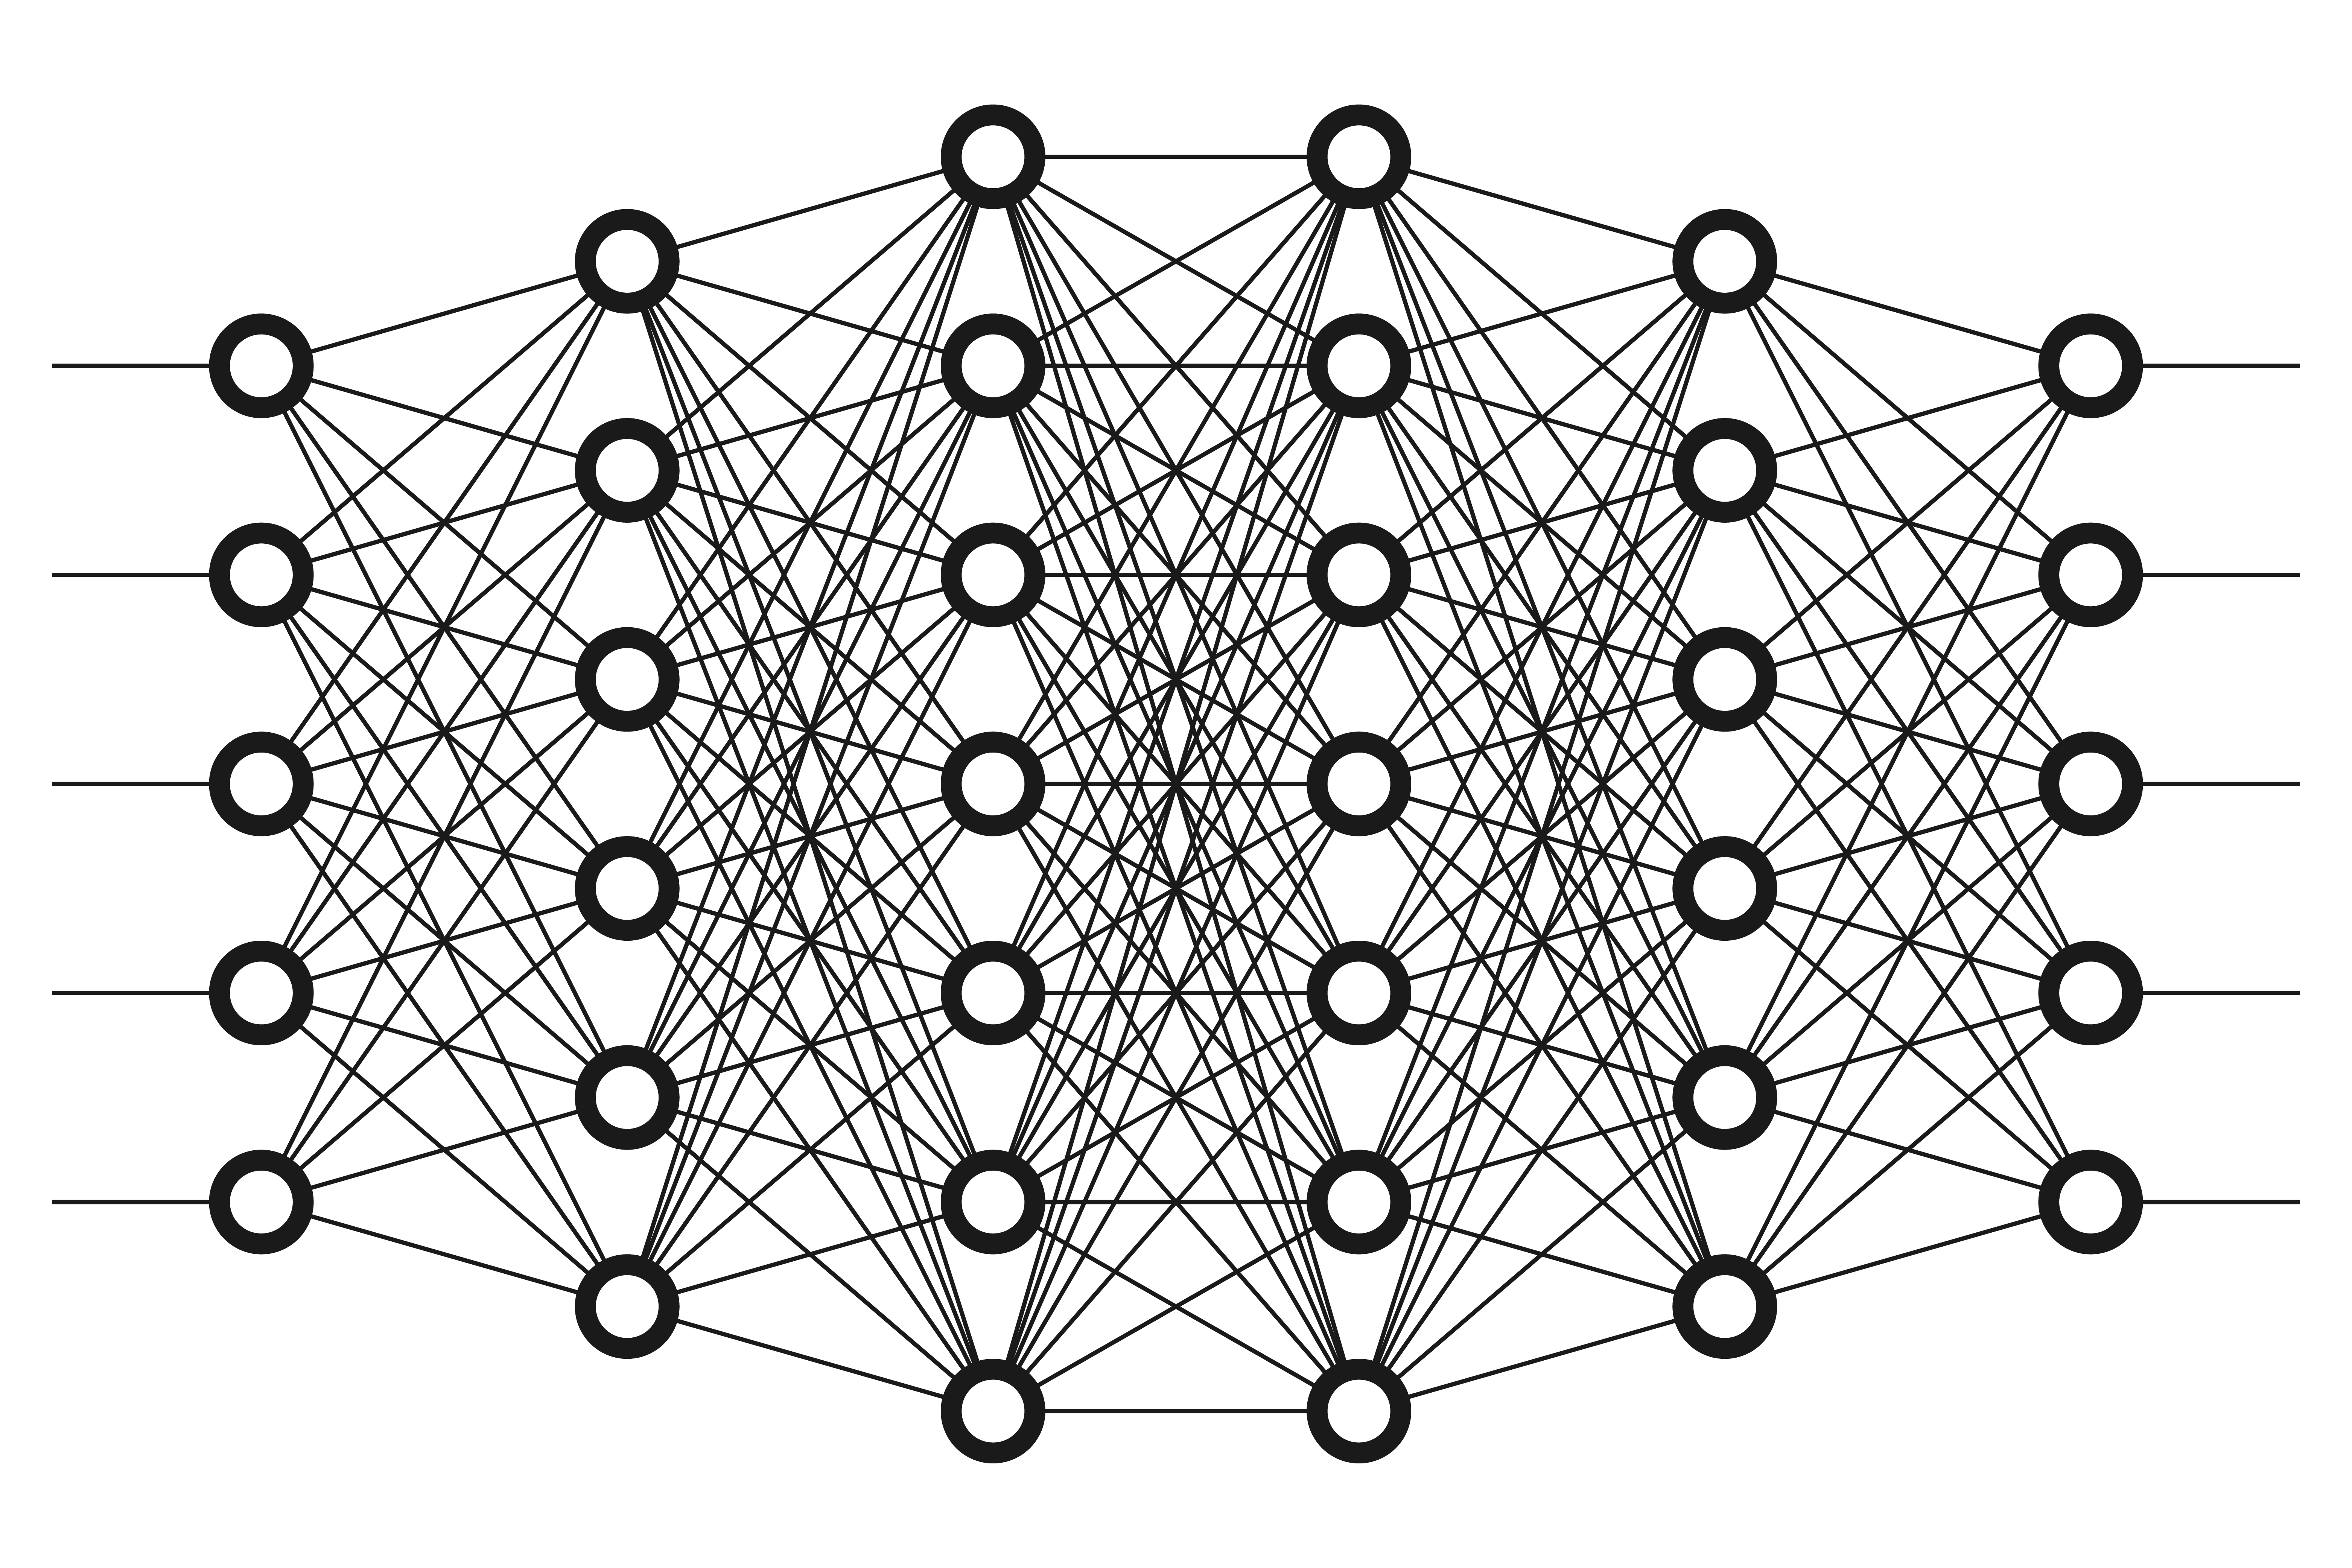
\includegraphics[width=\textwidth]{nn.png}};
	\end{tikzpicture}
\end{center}
\vfill
\begin{scriptsize}
Figure from [Katz et al., 2017]
\end{scriptsize}
\end{frame}
	
%%%%%%%%%%%%%%%%%%%%%%%%%%%%%%%%%%%%%%%%%%%%%%%%%%%%%%%%%%%

\begin{frame}{ReLU networks}

\begin{columns}
\begin{column}{0.6\textwidth}
Each hidden node (in purple) computes a weighted sum of its
	inputs on which it then applies the ReLU function to derive its
	output.
\end{column}
\begin{column}{0.3\textwidth}
	\scalebox{1}{
	\begin{tikzpicture}
		\node[draw=navyblue,fill=navyblue!5!white,rectangle,inner
		sep=0.2cm] (l)
	{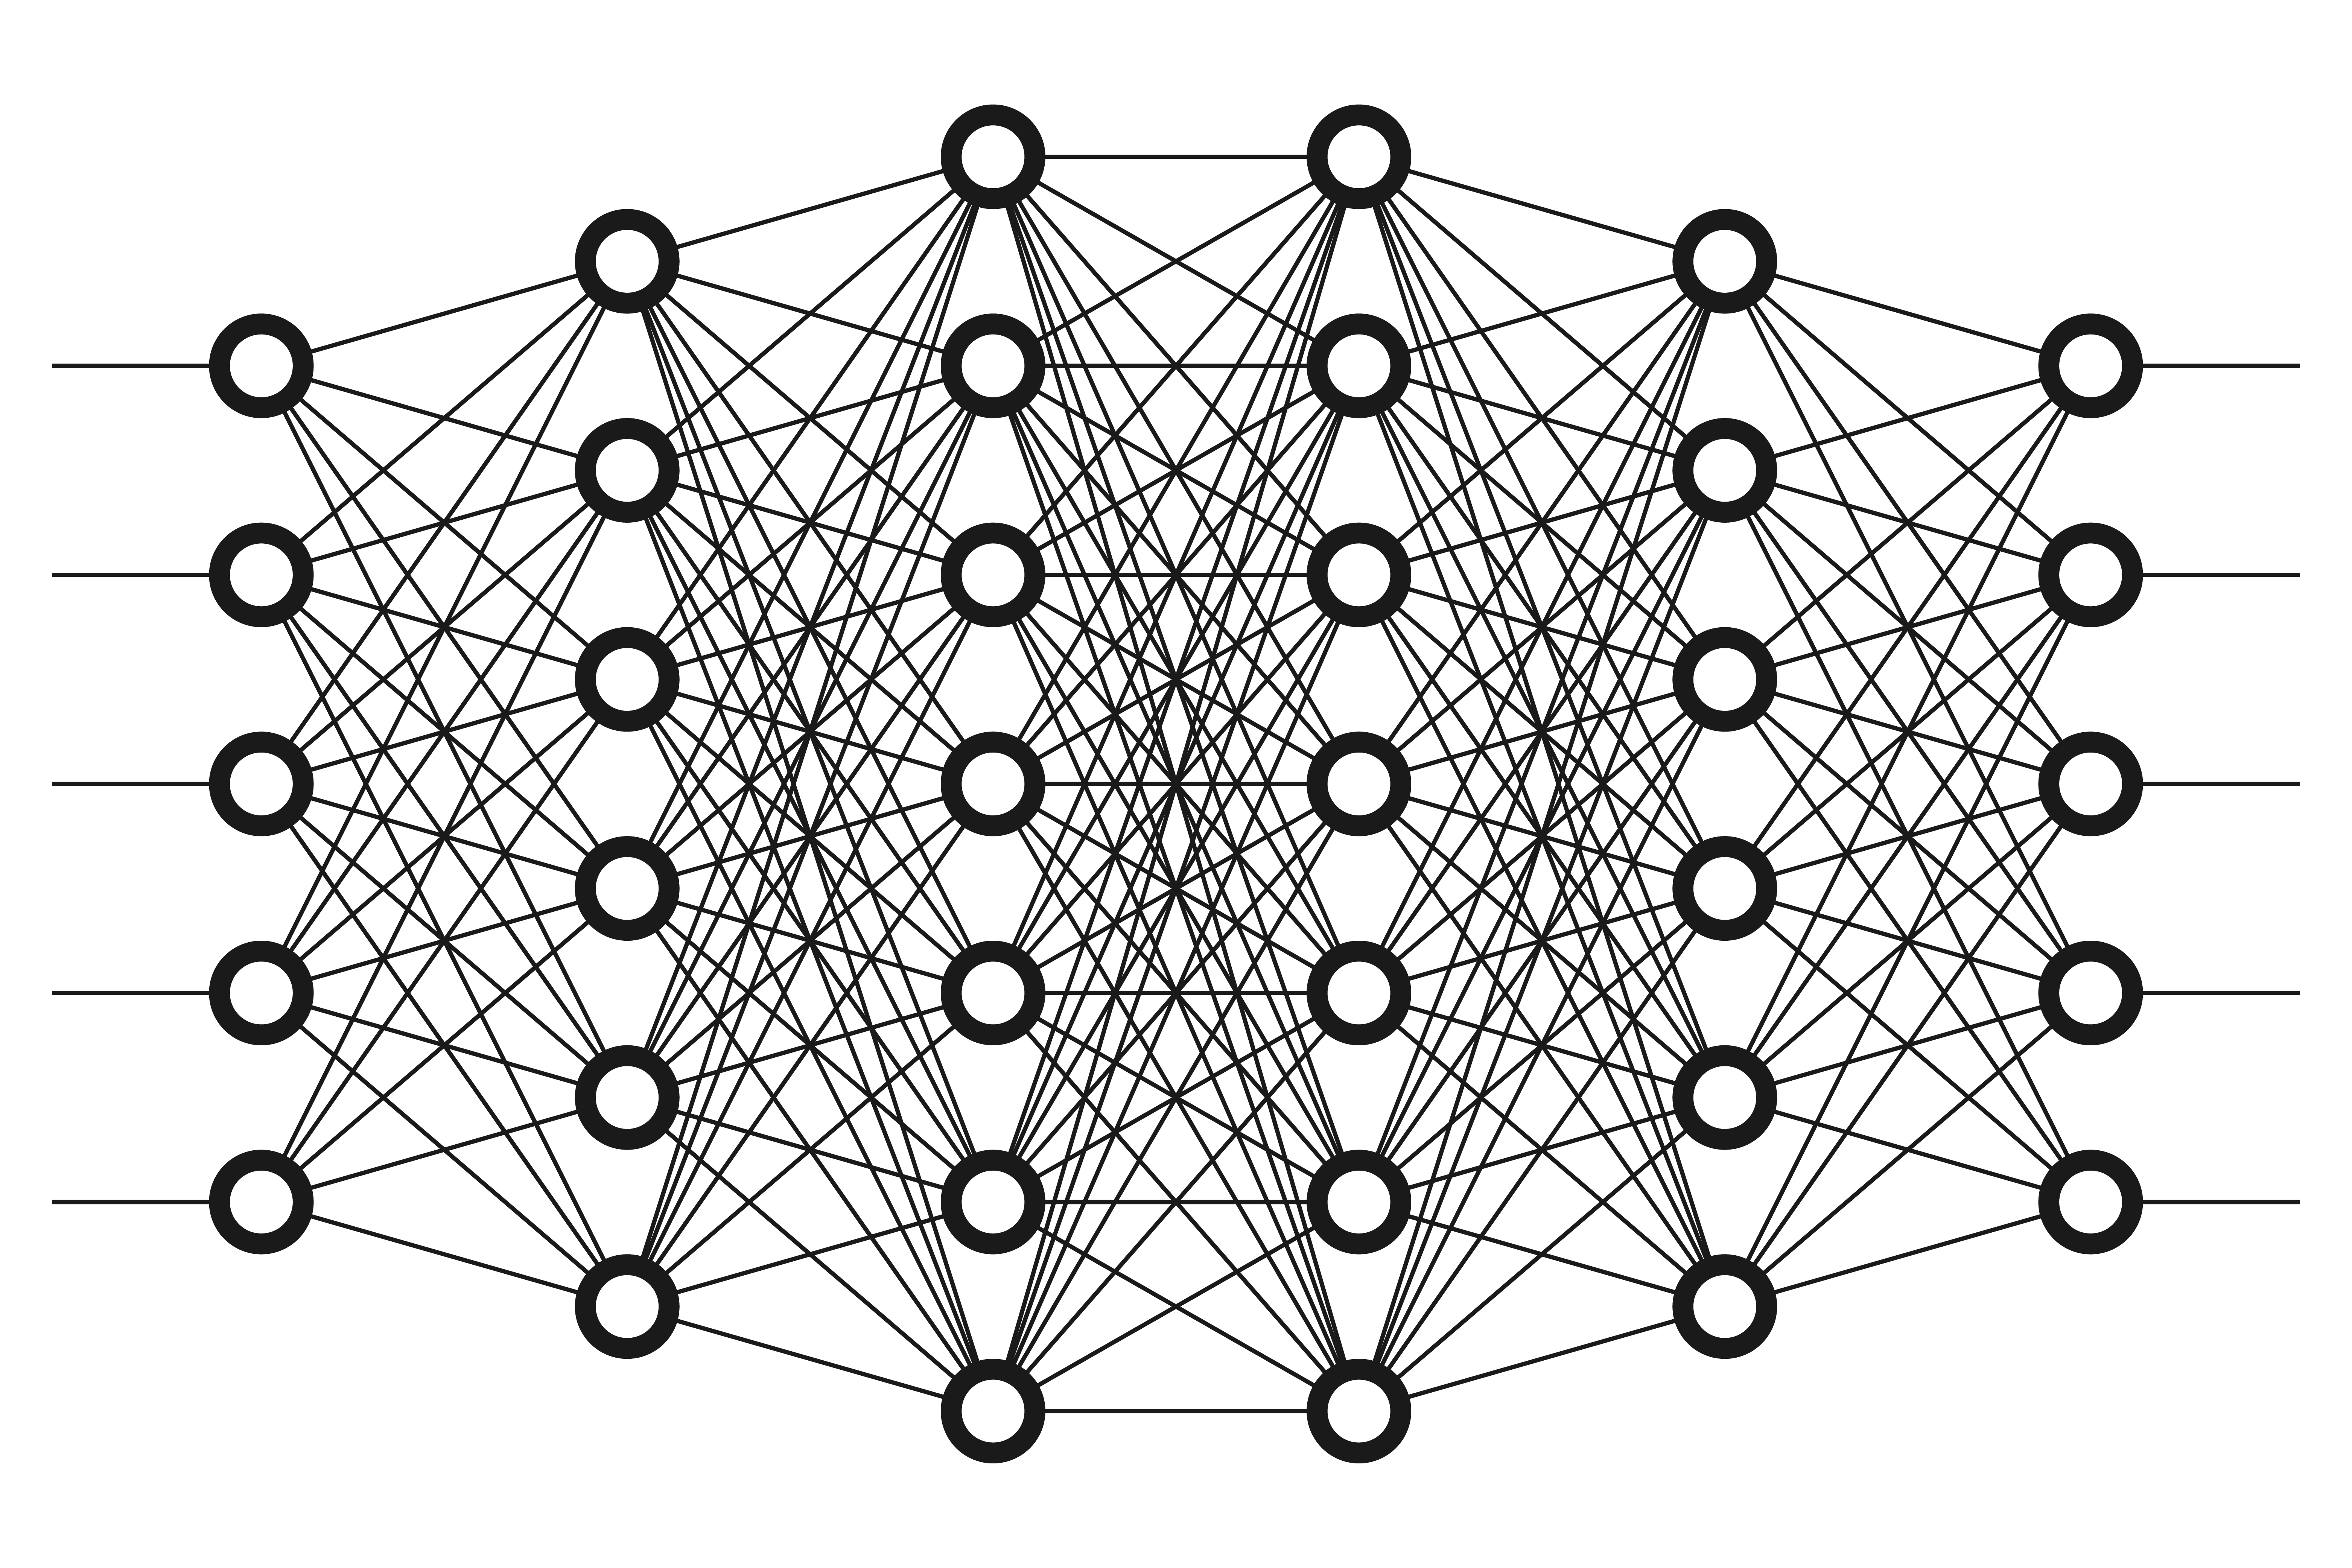
\includegraphics[width=\textwidth]{nn.png}};
	\end{tikzpicture}
	}
\end{column}
\end{columns}
\vspace{1em}


\begin{columns}
\begin{column}{0.6\textwidth}
\alert{ReLU function}: $\relu(x) = \max(x,0)$
\end{column}
\begin{column}{0.3\textwidth}
	\documentclass{standalone}
\usepackage[T1]{fontenc}
\usepackage{amsmath,amssymb,mathtools}
\newcommand{\set}[1]{\left\{ #1 \right \}}

\usepackage{graphicx}
\definecolor{navyblue}{RGB}{0,0,128}

\begin{document}

\begin{tikzpicture}[scale=0.85, every node/.style={transform shape}]
% horizontal axis
	\draw[->] (-3,0) -- (3,0) node[anchor=north] {$x$};

% vertical axis
	\draw[->] (0,-2) -- (0,2.2) node[anchor=east] {$\relu(x)$};

% labels
	\draw	(-2,0) node[anchor=south] {$l$}
	(2,0) node[anchor=north] {$u$};

\draw[very thick] (-2,0) -- (0,0);

%active state
\draw[very thick] (0,0) -- (2,2);
\draw[dotted] (2,0) -- (2,2);


% upper bound relaxation
\draw[draw=purple,fill=purple] (-2,0) circle (0.2em);
\draw[draw=purple,fill=purple] (2,0) circle (0.2em);


\end{tikzpicture}
\end{document}

\end{column}
\end{columns}
\vspace{1em}
ReLU is \alert{piecewise-linear}, hence ReLU networks are amenable to
\alert{complete verification}.
\end{frame}
	
%%%%%%%%%%%%%%%%%%%%%%%%%%%%%%%%%%%%%%%%%%%%%%%%%%%%%%%%%%%

\begin{frame}{Fragility of neural networks}

\begin{figure}
	\centering
	\resizebox{6cm}{!}{
	\begin{tikzpicture}[node distance=5cm,  minimum
	  height=0.7cm]

	%\node[draw=orange, fill=orange!10!white,rectangle,
	%xshift=0em, yshift=0cm, inner ysep=0.001cm] (1)
	%{  \includegraphics[width=0.05\textwidth]{mnist1.png}

	%};
	  \node[] (1)
	  {  \includegraphics[width=0.15\textwidth]{mnist1.png}
	};
	\node[right of =1, xshift=0.5cm] (2)
	{  \resizebox{5cm}{!}{
\begin{tikzpicture}[node distance=0.9cm,
	font=\scriptsize,auto,
	every node/.style={circle,inner sep=0.1cm},
	input/.style={fill=green,draw=green},
	hidden/.style={fill=black!50!white,draw=black!50!white},
	output/.style={fill=red,draw=red}]

  
  \node [input] (i1) {};
  \node [below of=i1, input] (i2) {};
  \node [below of=i2, input] (i3) {};
  \node [below of=i3, input] (i4) {};

  \node [right of = i1, above of = i1, xshift=1cm, hidden] (h11) {};
  \node [below of=h11, hidden] (h12) {};
  \node [below of=h12, hidden] (h13) {};
  \node [below of=h13, hidden] (h14) {};
  \node [below of=h14, hidden] (h15) {};
  \node [below of=h15, hidden] (h16) {};

  \node [right of = h11, xshift=1cm, hidden] (h21) {};
  \node [below of=h21, hidden] (h22) {};
  \node [below of=h22, hidden] (h23) {};
  \node [below of=h23, hidden] (h24) {};
  \node [below of=h24, hidden] (h25) {};
  \node [below of=h25, hidden] (h26) {};

  \node [right of = h21, xshift=1cm, hidden] (h31) {};
  \node [below of=h31, hidden] (h32) {};
  \node [below of=h32, hidden] (h33) {};
  \node [below of=h33, hidden] (h34) {};
  \node [below of=h34, hidden] (h35) {};
  \node [below of=h35, hidden] (h36) {};

  \node [right of = h32, xshift=1cm, output] (o1) {};
  \node [below of=o1, output] (o2) {};
  \node [below of=o2, output] (o3) {};
  \node [below of=o3, output] (o4) {};
  %\node [right of=1, xshift=-1.52m, fill=gray!50!white,draw=gray,neuron] (3) {};

  \foreach \i in {1,...,4}{
	  \draw[<-,color=black!30!white] (i\i) -- ++(-0.5,0);
	  \draw[->,color=black!30!white] (o\i) -- ++(0.5,0);
  }
  \foreach \i in {1,...,4}{
	 \foreach \j in {1,...,6}{
		 \draw [color=black!30!white]  (i\i) -- (h1\j);
   }}
  \foreach \i in {1,...,6}{
	 \foreach \j in {1,...,6}{
		 \draw [color=black!30!white]  (h1\i) -- (h2\j);
		 \draw [color=black!30!white]  (h2\i) -- (h3\j);
   }}
  \foreach \i in {1,...,6}{
	 \foreach \j in {1,...,4}{
		 \draw [color=black!30!white]  (h3\i) -- (o\j);
   }}

   %\node[below of=h16,xshift=-1cm,yshift=-0.5cm,input,label=right:{input node}] (inf1) {};
   %\node[right of=inf1,xshift=1.5cm,hidden,label=right:{hidden node}] (inf2) {};
   %\node[right of=inf2,xshift=1.5cm,output,label=right:{output node}] (inf3) {};

\end{tikzpicture}
}
 
		%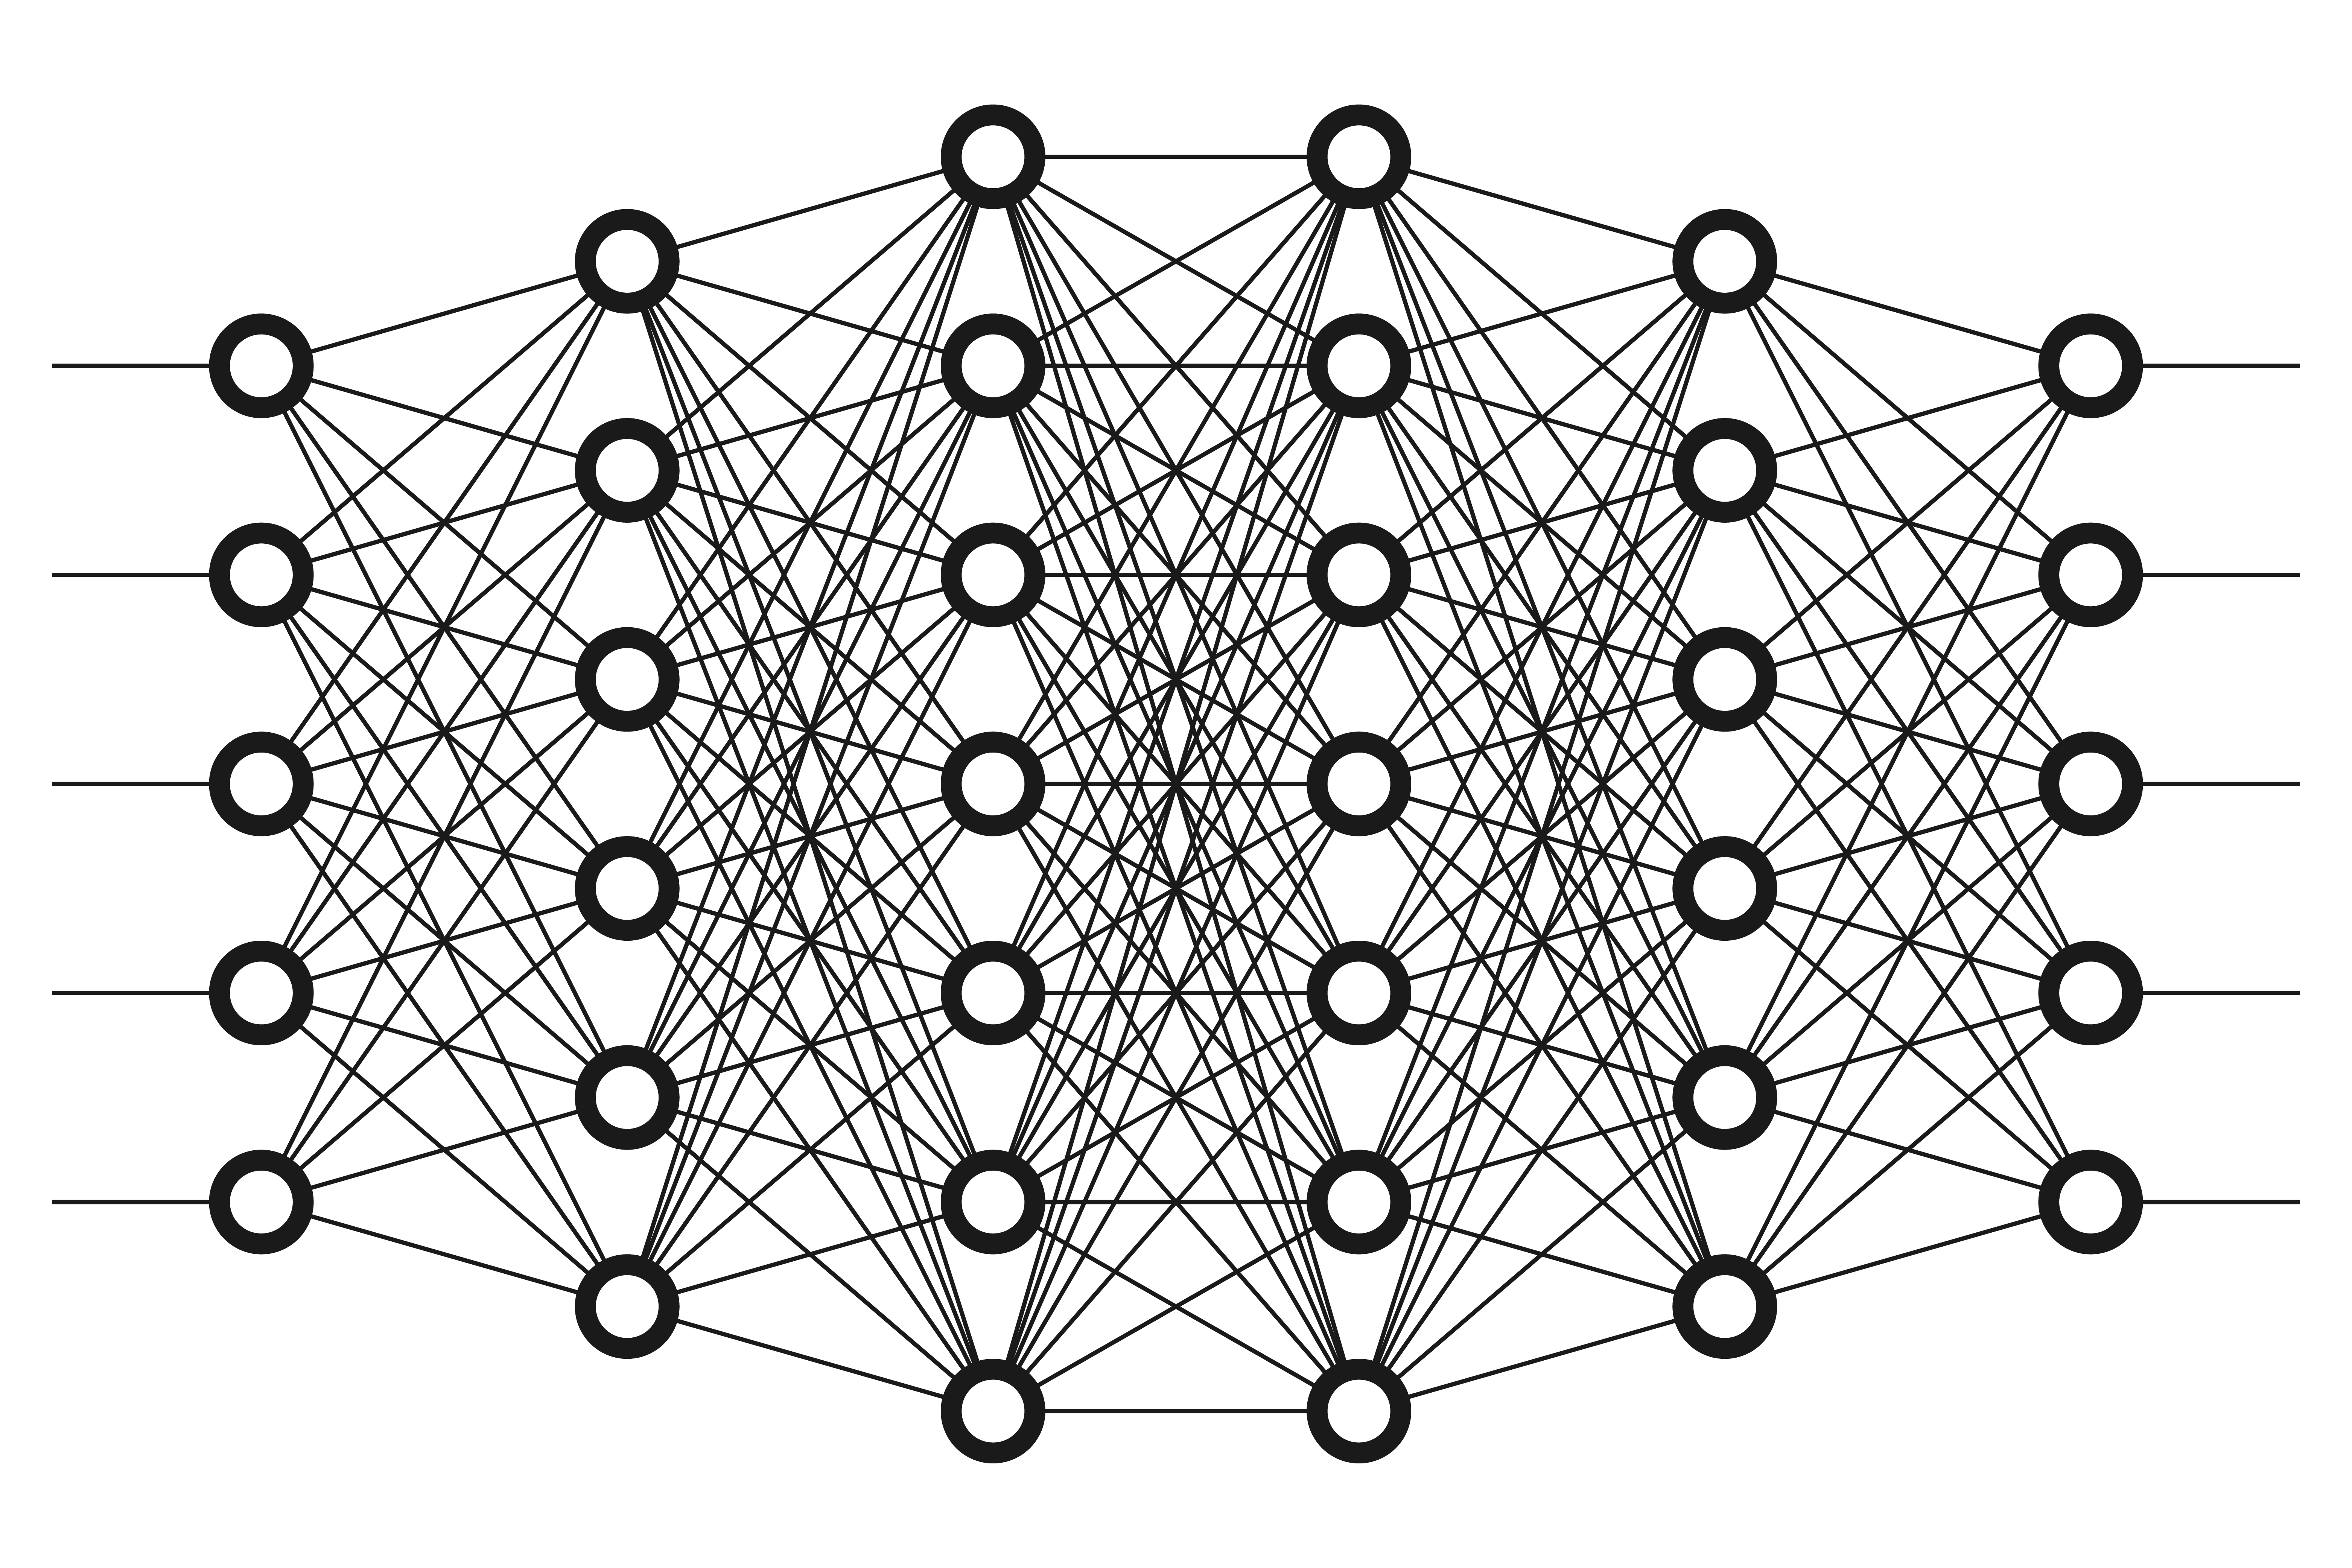
\includegraphics[width=0.6\textwidth]{nn.png}
	};
	\node[right of=2, xshift=-2em] (3) {{\Huge 2}};



	%\node[fit=(1)(2)(3), draw, navyblue, line width=0.03cm, solid, rounded corners,
	%inner sep=0.2cm] (s) {};


\path[->,very thick,every node/.style={->,font=\sffamily\normalsize}]
(1) edge node [] {} (2)
(2) edge node [] {} (3);

  \end{tikzpicture}
}




%%% Local Variables:
%%% mode: latex
%%% TeX-master: "deliverable-wp1.1-m18"
%%% fill-column: 79
%%% End:

\end{figure}

\end{frame}

%%%%%%%%%%%%%%%%%%%%%%%%%%%%%%%%%%%%%%%%%%%%%%%%%%%%%%%%%%%

\begin{frame}{Verification problem}

\begin{definition}[Verification problem.]
	Given a feed-forward ReLU neural  network $f \colon \mathbb R^{s_0}
	\rightarrow \mathbb{R}^{s_k}$, $\mathcal X \subseteq
	\mathbb R^{s_0}$, $\mathcal Y \subseteq \mathbb
	R^{s_k}$, check whether 
\[
	\forall  x \in \mathcal X  \colon f(x) \in
	\mathcal Y.
\]
\end{definition}

\vspace{2em}

\begin{itemize}  \itemsep 1em
	\item NP-complete [Katz et al., 2017], \alert{scalability} remains an issue.
	\item Need for novel methods tailored towards the exploitation of
		the highly structured nature of neural networks.
\end{itemize}

\end{frame}

%%%%%%%%%%%%%%%%%%%%%%%%%%%%%%%%%%%%%%%%%%%%%%%%%%%%%%%%%%%

\begin{frame}{Dependency analysis}

\begin{columns}
\begin{column}{0.5\textwidth}
\begin{block}{MILP compilation of a ReLU node}
		\vspace{-1.5em}
\begin{align*}
	&x \geq 0, \;\;\;\;\;\;\;\;\; x \geq \hat{x} \\
	&x \leq u \cdot \delta, \;\;\;\;\; x \leq \hat{x} - l \cdot (1 - \delta)
\end{align*}
where $x$ is the output of the node, $\hat{x}$ its
pre-activation, $l$ and $u$ are  lower and upper bounds of the pre-activation 
 and $\delta$ a
binary variable.
\end{block}
\end{column}
\begin{column}{0.5\textwidth}
\begin{block}{ReLU space}
	\begin{center}
	\resizebox{4.6cm}{!}{


\tikzset{cross/.style={cross out, draw=red, thick, minimum size=1.5em, inner sep=0pt, outer sep=0pt},
%default radius will be 1pt. 
cross/.default={1pt}}



\begin{tikzpicture}[node distance=3cm, font=\scriptsize,auto,
  neuron/.style={circle, inner sep=0.03cm}]


  \node [neuron,draw,xshift=7cm,yshift=0.2cm,draw=black,fill=black,text=white] (1) {$\node{1,2}$}
  child {node [neuron,draw=black,fill=black,text=white,yshift=0.3cm] (2) {$\node{2,1}$} 
    child {node [yshift=0.2cm] (4) {} edge from parent[dotted,thick]}
    child {node [yshift=0.2cm] (5) {} edge from parent[dotted,thick]}}
  child {node [neuron,draw,draw=black,fill=black,text=white,yshift=0.3cm] (3) {$\node{2,1}$} 
    child {node [yshift=0.2cm] (6) {} edge from parent[dotted,thick]}
    child {node [yshift=0.2cm] (7) {} edge from parent[dotted,thick]}};
  \path (1) -- (2) node [midway,left,xshift=-0em,yshift=0em] {$\it{inactive}$};
  \path (1) -- (3) node [midway,right,xshift=-0em,yshift=0em] {$\it{active}$};
  \path (2) -- (5) node [midway,right,xshift=-2em,yshift=-1em] {$\it{active}$};
  \path (3) -- (6) node [midway,left,xshift=2.5em,yshift=-1em] {$\it{inactive}$};
  \path (3) -- (7) node [midway,right,xshift=0.5em,yshift=-1em]
  {$\it{active}$};


\end{tikzpicture}
}


\end{center}
\end{block}
\end{column}
\end{columns}
\vspace{2em}
\alert{Dependency analysis} [AAAI19]:   Methods aiming at the
reduction of the ReLU space during branch-and-bound through the
exploitation of notions of dependencies between the nodes. \end{frame}

%%%%%%%%%%%%%%%%%%%%%%%%%%%%%%%%%%%%%%%%%%%%%%%%%%%%%%%%%%%

\begin{frame}{\texttt{Venus}}
	SoA sound and complete verification toolkit for ReLU networks
	\vspace{1em}
\begin{columns}
\begin{column}{0.5\textwidth}
\begin{figure}
\centering
\includegraphics[width=1.2\textwidth]{venus2.pdf}
\end{figure}
\end{column}
\begin{column}{0.5\textwidth}
\begin{figure}
\centering
\includegraphics[width=0.8\textwidth]{venus.pdf}
\end{figure}
\end{column}
\end{columns}
\vspace{1em}
Dependency analysis improves the performance of MILP-based
verification of neural networks.
\vspace{1em}

Venus outperforms the SoA by up to \alert{two orders of magnitude}
for perception networks.
\end{frame}

%%%%%%%%%%%%%%%%%%%%%%%%%%%%%%%%%%%%%%%%%%%%%%%%%%%%%%%%%%%

\begin{frame}{Neural-symbolic multi-agent systems}

\begin{figure}
	\centering
	\includegraphics[width=\textwidth]{cars.jpg}
\end{figure}

\end{frame}

%%%%%%%%%%%%%%%%%%%%%%%%%%%%%%%%%%%%%%%%%%%%%%%%%%%%%%%%%%%

\begin{frame}{Neural-symbolic multi-agent systems}

  \begin{block}{Verification problem}
	  Given a NMAS $\mathcal S$ and a temporal/strategic (CTL/ATL)
	  property $\varphi$, check whether every initial state in
  $\mathcal S$ 
	  satisfies $\varphi$.
  \end{block}

	
 	\vspace{3em}

  
  \begin{theorem}
	  Verifying NMAS against reachability properties (i.e., the system
	  eventually reaches an unsafe state) is undecidable [AAMAS20].
  \end{theorem}

\end{frame}

%%%%%%%%%%%%%%%%%%%%%%%%%%%%%%%%%%%%%%%%%%%%%%%%%%%%%%%%%%%

\begin{frame}{ Verification against bounded properties}


	Evaluation of \alert{bounded properties} concerns only a bounded number of
	time-steps from the evaluation state.

	E.g., \emph{bounded safety}: \[AG^k \mathit{safe} \triangleq
	AX^1\mathit{safe} \land AX^2 \mathit{safe} \land \dots \land AX^k
\mathit{safe}\]

  The verification problem for bounded properties admits a \alert{
  MILP representation}:
  \begin{columns}
   \begin{column}{0.5\textwidth}
	   \begin{block}{Monolithic encoding}
  	\centering
	\includegraphics[width=0.9\textwidth]{enc.png}
  \end{block}
  \end{column}
   \begin{column}{0.5\textwidth}
	   \begin{block}{Compositional encoding}
  	\centering
	\includegraphics[width=0.9\textwidth]{enc2.png}
  \end{block}
  \end{column}
  \end{columns}

\end{frame}

%%%%%%%%%%%%%%%%%%%%%%%%%%%%%%%%%%%%%%%%%%%%%%%%

\begin{frame}{Two agent aircraft collision avoidance}
  \begin{center}
	  \scalebox{0.8}{
    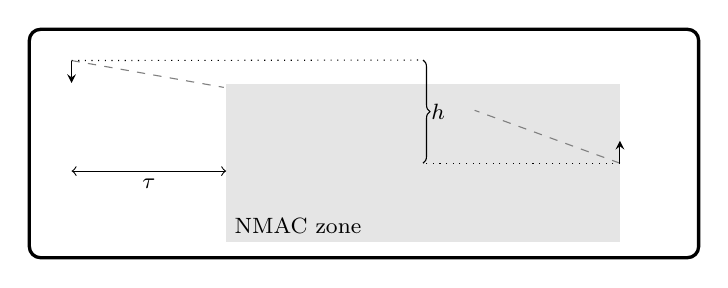
\begin{tikzpicture}%[remember picture, overlay, shift={(7.5,5.5)},xscale=0.5]
      \footnotesize
      \draw[rounded corners, very thick] (-0.5,-1.2) rectangle (8,1.7);
      \path[fill=gray!20] (2,-1) node[above right] {NMAC zone}%
      rectangle (7,1);

      \node[scale=1.5, rotate=-10, inner sep=0] (ownship) at (0,1.31) {\Plane};

      \node[scale=1.5, rotate=-20, xscale=-1, inner sep=0,red, anchor=east] (intruder) at (7,-0) {\Plane};

      \draw[dashed, gray] (intruder) -- ++(-20:-2);
      \draw[dashed, gray] (ownship) -- ++(-10:2);

      \coordinate (height) at (4.5,1.31);
      \draw[dotted] (ownship.0) -- (height);
      \draw[dotted] (intruder.0) -- (height|-intruder.0);
      \draw[decorate, decoration=brace] (height) -- node[right] {$h$}
      (height|-intruder.0);

      \coordinate (lower) at (2,-0.1);
      \draw[<->] (lower) -- node[below] {$\tau$} (ownship.0|-lower);

      \draw[-stealth] (ownship.0) -- ++(0,-0.285) node[right] {$\crown$};
      \draw[-stealth] (intruder.0) -- ++(0,0.285) node[above] {$\crint$};
	\end{tikzpicture}}
  \end{center}

  \begin{itemize} \itemsep 0.5cm
	\item Two aircraft: \alert{ownship} (black), \alert{intruder} (red).
	\item Each aircraft is controlled by a \alert{VerticalCAS system}
		(ReLU network), issuing an advisory for the range of
		accelerations the pilot should apply to avoid a {\em near
		min-air collision}.
	\item  We would like to establish that the ownship has a
strategy for the system to be in a safe configuration after~$k$ steps:

\[ \varphi_{1}^k = \egamma[\own]{k} \, \texttt{safe}\]
\end{itemize}
\end{frame}


%%%%%%%%%%%%%%%%%%%%%%%%%%%%%%%%%%%%%%%%%%%%%%%%


\begin{frame}{Experimental results}

\begin{tiny}

\small
\def\ctx{\color{red}}
\begin{center}
\begin{tabular}{c@{}c@{}c@{}c@{}c}
    \multicolumn{1}{c|}{} & \multicolumn{1}{c}{Parallel} & \multicolumn{1}{c}{Sequential} &  Monolithic \\\midrule
    \begin{tabular}{@{}c|}
      $h_I$ \\ 
      $\varphi^1$   \\
      $\varphi^2$   \\
      $\varphi^3$   \\\midrule
      $\psi^1$   \\
      $\psi^2$   \\
      $\psi^3$   
    \end{tabular}
 &
   \begin{tabular}{c@{~~}c@{~~}c|}
     95     & 100    & 105                          \\  
     2.636s & 2.698s & \ctx 3.042s  \\
     9.602s & 17.66s & \ctx 24.04s  \\
     414.1s & 384.7s & 393.9s  \\\midrule
     %
     93.30s & 111.1s & 4.178s  \\
     --     & 5871s  & 4497s  \\
     --     & --     &  --    
   \end{tabular}
 &
   \begin{tabular}{c@{~~}c@{~~}c|}
     95     & 100     & 105                         \\  
     1.426s & 1.464s  & \ctx  2.712s  \\
     5.005s & 26.15s  & \ctx 46.18s  \\
     1131s  & 1005.5s & 1027s  \\\midrule
     %
     1326s  & 1481s   &  5.370s  \\
     --     & --      &  --   \\
     --     & --      & --
   \end{tabular}
 &
   \begin{tabular}{c@{~~}c@{~~}c|}
     95     & 100    & 105  \\  
     0.253s & 0.212s & \ctx 83.93s\\
     84.45s & 47.65s & -- \\
     --     & --     & -- \\\midrule
     %
     1511s & 1182s &  4.498s \\
     -- & -- &  -- \\
     -- & -- &  -- 
   \end{tabular}
\end{tabular}
\end{center}

\end{tiny}

\begin{itemize}
	\item Parallel approaches particularly suitable for identifying
		\alert{shallow bugs}.
	%\item  Verification times grow exponentially with the number of
		%steps. 
	\item \alert{Bottleneck}: state space of the associated temporal model +
		evaluation of atomic propositions.
\end{itemize}

\end{frame}

%%%%%%%%%%%%%%%%%%%%%%%%%%%%%%%%%%%%%%%%%%%%%%%%

\begin{frame}{Future work}	
  
	{\bf Scalability}

  \begin{center}
	\vspace{-1em}
  \begin{tikzpicture}[%
    >=stealth,
	node distance=4cm,
    on grid,
    auto
  ]
	\begin{scriptsize}
		\node [text width=3.5cm] (1)  {
			\begin{block}{{\footnotesize Neural agents}}
		\begin{itemize}
			\item	Up to 2018: $10^1$
			\item 2018-2020 (VNN20):  $10^4$
			\item 2020-2022: $10^6$ (?)
		\end{itemize}
  	  \end{block}
  };

  \node [right of = 1,text width=3cm] (2){
	  \begin{block}{{\footnotesize Neural-symbolic MAS}}
		\begin{itemize}
			\item $10^2$ nodes
			\item $10^1$ time-steps
		\end{itemize}
		\end{block}
  };

  \node [right of = 2, xshift=-4.5em,text width=1.5cm] (3){
	  \begin{block}{{\footnotesize Neural swarms}}
		\begin{itemize}
			\item (?)
		\end{itemize}
		\end{block}
  };

  \path[->,line width=2]
	(1) edge (2)
	(2) edge (3);
	\end{scriptsize}
  \end{tikzpicture}	

	\end{center}

{\bf Analysis of industrial models}

	\begin{footnotesize}
\begin{itemize}
	\item Perception modules for autonomous driving.
	\item Classification/localisation/segmentation models for deep
		learning.
\end{itemize}


\end{footnotesize}
	{\bf Repair and data augmentation}
	\begin{footnotesize}
	\begin{itemize}
		\item Analysis of counterexamples to repair faulty models.
		\item Augmentation of the training set with counterexamples
			and retraining of the models.
	\end{itemize}
	\end{footnotesize}




{\bf Other instantiations of the overall verification problem (?)}
	\begin{footnotesize}
\begin{itemize}
	\item DAI, Planning
\end{itemize}
\end{footnotesize}
		
\end{frame}


%%%%%%%%%%%%%%%%%%%%%%%%%%%%%%%%%%%%%%%%%%%%%%%%

\begin{frame}{Future work}

\begin{block}{Scalable verification of neural agents.}
\begin{itemize}
	\item Linear approximations of ReLUs
	\item Dependency-based branching methods
	\item Structural abstractions in CEGAR frameworks.
\end{itemize}
\end{block}

\begin{exampleblock}{Neural-symbolic MAS}
\begin{itemize}
	\item Abstractions on the induced temporal models.
	\item Compositional Reasoning.
\end{itemize}
\end{exampleblock}

\begin{alertblock}{Neural-symbolic swarms}
	\begin{itemize}
		\item Cutoffs.
		\item Counter abstractions.
	\end{itemize}
\end{alertblock}
\end{frame}


%%%%%%%%%%%%%%%%%%%%%%%%%%%%%%%%%%%%%%%%%%%%%%%%

\begin{frame}{RAP and DAI}

{\bf RAP}

\begin{itemize} \itemsep 0.2cm
	\item Planning in Neural MAS via formal verification.
	\item  Translations of argumentation frameworks into temporal
		models and formalisation of argumentation properties into
		temporal and strategy logics.
\end{itemize}

\vspace{1em}

{\bf DAI}
\begin{itemize} \itemsep 0.2cm
	\item Parameterised verification for the analysis of emergent
		behaviours in DAI protocols  (multi-party negotiation
		protocols and auctions, voting protocols, e-services).

	\item Formal verification of neural normative MAS against deontic
		specifications.
\end{itemize}

\end{frame}

\end{document}
